\section{Discussion}

\subsection{Task 1: \cartpole with vanilla DQN}

\subsubsection{Training Commands}

For the task 1, which required to use the vanilla DQN algorithm, I used the following command to train the agent:

\begin{minted}{bash}
     python3 trainer.py --env cartpole --exp report --vanilla --epsilon-decay 0.99
\end{minted}

The command specifies the environment as \cartpole, the experiment name as \texttt{report}, and the epsilon decay rate as 0.99.
The \texttt{----vanilla} flag indicates that the agent should use the vanilla DQN algorithm without any modifications. This will (1) set the \texttt{PER alpha} and \texttt{PER beta} hyperparameters to $0$ and $1$, respectively, which means that the agent will not use prioritized experience replay, (2) set the \texttt{N Steps} hyperparameter to $1$, which means that the agent will use one-step Q-learning updates, and (3) set the \texttt{Update Period} hyperparameter to $1$, which means that the agent will update the model after every step to discard the effect of the target network.
The \texttt{----epsilon-decay} flag specifies the decay rate for the epsilon value, which controls the exploration-exploitation trade-off during training.
The other hyperparameters are set to their default values.

The hyperparameters values are as follows:
\begin{itemize}
    \item \textbf{Batch size}: $32$
    \item \textbf{Discount factor}: $0.99$
    \item \textbf{Learning rate}: $0.0001$
    \item \textbf{Memory size}: $100,000$
    \item \textbf{Epsilon start}: $1$
    \item \textbf{Epsilon decay}: $0.99$
    \item \textbf{Epsilon min}: $0.015$
    \item \textbf{PER alpha}: $0$
    \item \textbf{PER beta}: $1$
    \item \textbf{N Steps}: $1$
    \item \textbf{Update Period}: $1$
    \item \textbf{Number of episodes}: $500$
    \item \textbf{Seed}: $42$
    \item \textbf{Evaluation episodes}: $10$
\end{itemize}

The training process consists of $500$ episodes, and the evaluation reward is calculated as the average reward over $10$ evaluation episodes.
The training process is performed using the \texttt{Trainer} class, which handles the training loop and updates the model.

\subsubsection{Training Curves}

The training curves for the task 1 are shown in Figure \ref{fig:cartpole-training-curve}.

\begin{figure}[H]
    \centering
    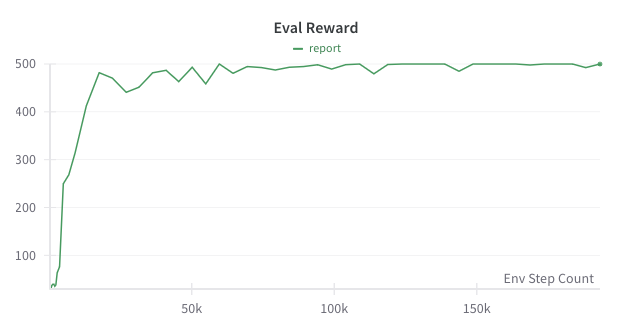
\includegraphics[width=0.8\textwidth]{figures/task1.png}
    \caption{Training curves for the \cartpole environment.}
    \label{fig:cartpole-training-curve}
\end{figure}

\subsubsection{Testing Commands}

We can test the trained agent using the following command:
\begin{minted}{bash}
     python3 tester.py --env cartpole --exp report --model ./results/cartpole/report/best_model.pt --episodes 30
\end{minted}

This can achieve the score over than $480$ in 30 consecutive episodes.

\subsection{Task 2: \pong with vanilla DQN}

\subsubsection{Training Commands}

For the task 2, which required to use the vanilla DQN algorithm, I used the following command to train the agent:

\begin{minted}{bash}
     python3 trainer.py --env pong --exp report --vanilla --episodes 2500 --eval-episodes 2
\end{minted}

The command specifies the environment as \pong, the experiment name as \texttt{report}, and the \texttt{----vanilla} flag indicates that the agent should use the vanilla DQN algorithm without any modifications. This will (1) set the \texttt{PER alpha} and \texttt{PER beta} hyperparameters to $0$ and $1$, respectively, which means that the agent will not use prioritized experience replay, (2) set the \texttt{N Steps} hyperparameter to $1$, which means that the agent will use one-step Q-learning updates, and (3) set the \texttt{Update Period} hyperparameter to $1$, which means that the agent will update the model after every step to discard the effect of the target network.
The \texttt{----episodes} flag specifies the maximum number of episodes for training, which is set to $2500$ in this case.
The \texttt{----eval-episodes} flag specifies the number of evaluation episodes, which is set to $2$ in this case.
The other hyperparameters are set to their default values.
The hyperparameters values are as follows:
\begin{itemize}
    \item \textbf{Batch size}: $32$
    \item \textbf{Discount factor}: $0.99$
    \item \textbf{Learning rate}: $0.0001$
    \item \textbf{Memory size}: $100,000$
    \item \textbf{Epsilon start}: $1$
    \item \textbf{Epsilon decay}: $0.99999$
    \item \textbf{Epsilon min}: $0.005$
    \item \textbf{PER alpha}: $0$
    \item \textbf{PER beta}: $1$
    \item \textbf{N Steps}: $1$
    \item \textbf{Update Period}: $1$
    \item \textbf{Number of episodes}: $500$
    \item \textbf{Seed}: $42$
    \item \textbf{Evaluation episodes}: $2$
\end{itemize}

\subsubsection{Training Curves}

\subsubsection{Testing Commands}

\subsection{Task 3: \pong with DQN Variants}

\subsubsection{Training Commands}

For the task 3, which required to use the DQN variants.

However, I use the vanilla DQN algorithm for the \pong environment and \textbf{it can \textcolor{red}{achieve the score of $21$} (evaluated in 30 consecutive episodes) in about \textcolor{red}{$140k$ environment steps}}.

The training commands are as follows:

\begin{minted}{bash}
     python3 trainer.py --env pong --exp task3 --vanilla
\end{minted}

The command specifies the environment as \pong, the experiment name as \texttt{task3}, and the \texttt{----vanilla} flag indicates that the agent should use the vanilla DQN algorithm without any modifications. This will (1) set the \texttt{PER alpha} and \texttt{PER beta} hyperparameters to $0$ and $1$, respectively, which means that the agent will not use prioritized experience replay, (2) set the \texttt{N Steps} hyperparameter to $1$, which means that the agent will use one-step Q-learning updates, and (3) set the \texttt{Update Period} hyperparameter to $1$, which means that the agent will update the model after every step to discard the effect of the target network.

The other hyperparameters are set to their default values.
The hyperparameters values are as follows:
\begin{itemize}
    \item \textbf{Batch size}: $32$
    \item \textbf{Discount factor}: $0.99$
    \item \textbf{Learning rate}: $0.0001$
    \item \textbf{Memory size}: $100,000$
    \item \textbf{Epsilon start}: $1$
    \item \textbf{Epsilon decay}: $0.99999$
    \item \textbf{Epsilon min}: $0.005$
    \item \textbf{PER alpha}: $0$
    \item \textbf{PER beta}: $1$
    \item \textbf{N Steps}: $1$
    \item \textbf{Update Period}: $1$
    \item \textbf{Number of episodes}: $500$
    \item \textbf{Seed}: $42$
    \item \textbf{Evaluation episodes}: $10$
\end{itemize}

\subsubsection{Training Curves}

The training curves for the task 3 are shown in Figure \ref{fig:pong-task3-training-curve}.
\begin{figure}[H]
    \centering
    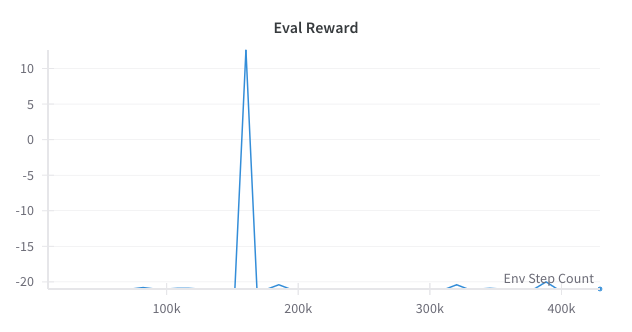
\includegraphics[width=0.8\textwidth]{figures/task3.png}
    \caption{Training curves for the \pong environment.}
    \label{fig:pong-task3-training-curve}
\end{figure}

We can see that the evaulation result shows that the agent can not achieve well performance in the \pong environment. It always get the score of $-21$ except a special snapshot that the agent can get the score over than $10$.
By the way, this evaluation score during the training process is the average score of 10 episodes.

After inspecting the special snapshot, I found that the agent can get the score of $21$ in some episodes by moving to a specific position and hitting the ball at the right time without moving the paddle again.
However, in the other episodes, the agent can not hit any ball and the score is $-21$.

\subsubsection{Testing Commands}

Therefore, during the testing process, if we use this snapshot to test the agent in the \pong environment, the agent can get the score of $21$ in 30 consecutive episodes by the following testing command:
\begin{minted}{bash}
     python3 tester.py --env pong --exp task3 --model ./results/pong/task3/best_model.pt --seed 92439410 --episodes 30
\end{minted}

The command specifies the environment as \pong, the experiment name as \texttt{task3}, and the \texttt{----model} flag indicates that the agent should use the model saved in the \texttt{best\_model.pt} file, you should change the path to your own path.
The \texttt{----seed} flag specifies the first random seed for the environment, and the following seed for the environment will be $seed + \text{episode\_number}$. That is to say, the first episode will use the seed $92439410$, the second episode will use the seed $92439411$, and so on.
The \texttt{----episodes} flag specifies the number of evaluation episodes, which is set to $30$ in this case.



\subsection{Analyze each Technique}
